\section{Данные и списки}
\subsection{Данные}
\subsubsection{Сущности}

Для реализации необходимы сущности:
\begin{enumerate}
  \item Задача;
  \item Раздел;
  \item Пособие;
  \item Презентация;
  \item Пользователь;
  \item Группа;
  \item Привелегии;
\end{enumerate}

\paragraph{Сущность ЗАДАЧА} необходима для отображения различных заданий. ЗАДАЧА -- основная сущность в данной системе. Она должна иметь следующие параметры:
\begin{enumerate}
  \item Заголовок
  \item Условие
  \item Решение
  \item Ответ
  \item Сложность
\end{enumerate}

\paragraph{Сущность РАЗДЕЛ} агрегирует задачи и разделы. РАЗДЕЛ позволяет создать иерархию любой вложенности. Основные параметры:
\begin{enumerate}
  \item Заголовок
  \item Родительский раздел
  \item Вложенные задачи
\end{enumerate}

\paragraph{Сущность ПОСОБИЕ} необходима для предоставления информации и скачивания пособий с сайта. Необходимые параметры:
\begin{enumerate}
  \item Заголовок
  \item Ссылка для скачивания
\end{enumerate}

\paragraph{Сущность ПРЕЗЕНТАЦИЯ} необходима для передоставления информации и скачивания презентации в двух форматах:
\begin{enumerate}
  \item PDF
  \item PPTX
\end{enumerate}
ПРЕЗЕНТАЦИЯ должна содержать параметры:
\begin{enumerate}
  \item Заголовок
  \item Ссылка на скачивания PDF
  \item Cсылка на скачивание PPTX
\end{enumerate}

\paragraph{Сущность ПОЛЬЗОВАТЕЛЬ} необходима для регистрации и авторизации на административной части сайта.
ПОЛЬЗОВАТЕЛЬ должен содержать параметры:
\begin{enumerate}
  \item Имя
  \item E-mail
  \item Пароль
  \item Группа, к которой принадлеит
\end{enumerate}

\paragraph{Сущность ГРУППЫ} необходима для разделения пользователей на группы с различными правами на сайте. Изначально в системе закладывается два типа пользователей:
\begin{enumerate}
  \item Гость -- права просмотра
  \item Администратор -- права просмотра и редактирования
\end{enumerate}
ГРУППА должна содержать параметры:
\begin{enumerate}
  \item Название
  \item Список привилегий
\end{enumerate}

\paragraph{Сущность ПРИВЕЛЕГИИ} необходимо для абстракции и дальнейшей агрегации привилегий по типу, например:
\begin{enumerate}
  \item Чтение;
  \item Редактирование;
\end{enumerate}
Сущность ПРИВИЛЕГИЯ содержит параметры:
\begin{enumerate}
  \item Имя;
\end{enumerate}

\subsubsection{База данных}
Схема БД:
\begin{figure}[H]
  \begin{center}
    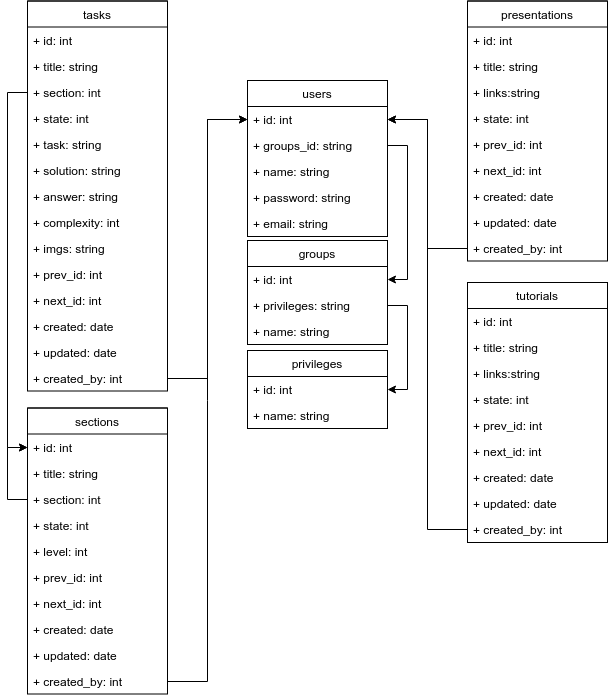
\includegraphics[width=0.5\textwidth]{6-index-1}
  \end{center}
\end{figure}
\begin{enumerate}
  \item tasks;
  \item section;
  \item tutorial;
  \item presentation;
  \item users;
  \item groups;
  \item privileges;
\end{enumerate}

\paragraph{TASK} таблица хранящая в себе сущности типа "ЗАДАЧА". Структура таблицы:
\begin{enumerate}
  \item id
  \item title
  \item section
  \item state
  \item task
  \item solution
  \item answer
  \item imgs
  \item complexity
  \item prev\_id
  \item next\_id
  \item created
  \item updated
\end{enumerate}

\subparagraph{id} -- уникалный идентификатор задачи или системный номер.
\subparagraph{title} -- заголовок или название задачи.
\subparagraph{section} -- id раздела, которому принадлежит задача.
\subparagraph{state} -- состояние задачи:
\begin{itemize}
  \item Опубликовано ($1$) -- доступна для просмотра
  \item Не опубликовано ($0$) -- скрыта для просмотра
\end{itemize}
\subparagraph{task} -- условие задачи.
\subparagraph{solution} -- решение задачи.
\subparagraph{answer} -- ответ задачи.
\subparagraph{imgs} -- прикрепленные изображения.
\subparagraph{complexity} -- сложность задачи.
\subparagraph{prev id} -- id предыдущей задачи.
\subparagraph{next id} -- id следующей задачи.
\subparagraph{created} -- дата создания.
\subparagraph{updated} -- дата редактирования.

\paragraph{SECTION} -- таблица, хранящая сущности "РАЗДЕЛ". Структура таблицы:
\begin{enumerate}
  \item id
  \item title
  \item section
  \item state
  \item prev\_id
  \item next\_id
  \item level
  \item created
  \item updated
\end{enumerate}

\subparagraph{id} -- уникальный идентификатор или системный номер раздела.
\subparagraph{title} -- заголовок или название раздела.
\subparagraph{section} -- id родительского раздела.
\subparagraph{state} -- состояние раздела:
\begin{itemize}
  \item Опубликовано ($1$) -- доступен для просмотра
  \item Не опубликовано ($0$) -- скрыт для просмотра
\end{itemize}
\subparagraph{prev id} -- id предыдущего раздела.
\subparagraph{next id} -- id следующего раздела.
\subparagraph{level} -- уровень вложенности раздела.
\subparagraph{created} -- дата создания.
\subparagraph{updated} -- дата последнего обновления.

\paragraph{TUTORIAL} -- таблица, хранящая сущность "ПОСОБИЕ". Структура таблицы:
\begin{enumerate}
  \item id
  \item title
  \item links
  \item prev\_id
  \item next\_id
  \item created
  \item updated
\end{enumerate}
\subparagraph{ id } -- уникальный идентификатор или системный номер.
\subparagraph{title} -- заголовок или название.
\subparagraph{links} -- ссылки для скачивания.
\subparagraph{prev id} -- id предыдущего.
\subparagraph{next id} -- id следующего.
\subparagraph{created} -- дата создания.
\subparagraph{updated} -- дата последнего изменения.

\paragraph{PRESENTATION}
\begin{enumerate}
  \item id
  \item title
  \item links
  \item prev\_id
  \item next\_id
  \item created
  \item updated
\end{enumerate}
\subparagraph{ id } -- уникальный идентификатор или системный номер.
\subparagraph{title} -- заголовок или название.
\subparagraph{links} -- ссылки для скачивания.
\subparagraph{prev id} -- id предыдущего.
\subparagraph{next id} -- id следующего.
\subparagraph{created} -- дата создания.
\subparagraph{updated} -- дата последнего изменения.

\paragraph{USERS} -- таблица, хранящая сущности "ПОЛЬЗОВАТЕЛЬ". Структура таблицы:
\begin{enumerate}
  \item id
  \item name
  \item psswd
  \item rights
\end{enumerate}
\subparagraph{id} -- уникальный идентификатор или системное имя.
\subparagraph{name} -- имя пользователя.
\subparagraph{groups id} -- идентификаторы груп.
\subparagraph{password} -- пароль пользователя.
\subparagraph{email} -- электронная почта пользователя.

\paragraph{GROUPS} -- таблица, хранящая сущности "ГРУППЫ". Структура таблицы:
\begin{enumerate}
  \item id
  \item name
  \item privileges
\end{enumerate}
\subparagraph{id} -- уникальный индентификатор или системное имя;
\subparagraph{name} -- название группы;
\subparagraph{privileges} -- id привилегий.

\paragraph{PRIVILEGES} -- таблица, хранящая сущности "ПРИВИЛЕГИИ". Структура таблицы:
\begin{enumerate}
  \item id
  \item name
\end{enumerate}
\subparagraph{id} --  уникальный индентификатор или системное имя;
\subparagraph{name} -- имя привелегии;

\subsection{Списки}
Для предоставление информации клиентам и администратору используются списки:
\subsubsection{Списки клиентской части}
\begin{enumerate}
  \item Раздел ЕГЭ базового уровня и его подразделы
  \item Раздел ЕГЭ профильного уровня и его подразделы
  \item Раздел ОГЭ и его подразделы
  \item Раздел Высшей математики
  \item Cписки задача
  \item Презентации
  \item Пособия
  \item Генератор вариантов
\end{enumerate}

\paragraph{Список разделы} агрегирует:
\begin{enumerate}
  \item Раздел ЕГЭ базового уровня и его подразделы
  \item Раздел ЕГЭ профильного уровня и его подразделы
  \item Раздел ОГЭ и его подразделы
  \item Раздел Высшей математики
\end{enumerate}
Данные списки разделов имеют общую структуру. При клике на один из разделов, мы переходим к списку дочерних разделов, при клике на которые мы получим такие дочерние списки подразделов или списки задач.

\paragraph{Список задач} -- это череда идущих друг за другом задач, которые принадлежат одному разделу. Список состоит из сущностей "ЗАДАЧА". Клиент должен видеть:
\begin{enumerate}
  \item Условие
  \item Решение
  \item Ответ
  \item Сложность
  \item Заголовок
  \item Уникальный идентификатор задачи
\end{enumerate}
В списке изначально скрыты "ответ" и "решение". При клике на соответствующие элементы управления клиент должен увидеть скрытые поля "ответ" и "решение".

\paragraph{Презентации и пособия} состоят из сущностей "ПРЕЗЕНТАЦИЯ" и "ПОСОБИЕ" соответсвенно. Клиент видит список заголовков и ссылки на скачивание.

\paragraph{Генератор вариантов} -- программный продукт, результатом работы которого является список сущностей "ЗАДАЧА". В отличии от "СПИСОК ЗАДАЧ" сущности принадлежат различным разделам.
\subparagraph{Алгоритм:} ...

\subsubsection{Списки администратора}
\begin{enumerate}
  \item Список задачи
  \item Список раздела
  \item Список пособия
  \item Список презентации
  \item Список задач
  \item Список разделов
  \item Список пособий
  \item Cписок перезентаций
\end{enumerate}

\paragraph{Список задачи} -- форма создания/редактирования задачи.
Процесс создания/редактирования задачи заключается в ручном заполнении параметров сущности "ЗАДАЧА". Администратоту необходимо заполить:
\begin{enumerate}
  \item Заголовок (title)
  \item Родительский раздел (section)
  \item Состояние (state)
  \item Следует за (prev\_id)
  \item Сложность (complexity)
  \item Условие (task)
  \item Решение (solution)
  \item Ответ (answer)
  \item Изображения (imgs)
  \item Порядковый номер (order)
\end{enumerate}
\subparagraph{ПОРЯДОК} -- вычисляемый параметр, который отображает позицию задачи в общем списке.

\paragraph{Список раздела} -- форма создания/редактирования раздела.
Процесс создания/редактирования раздела заключается в ручном заполнении сущности "РАЗДЕЛ".
Необходимо заполнить:
\begin{enumerate}
  \item Заголовок (title)
  \item Родительский раздел (section)
  \item Состояние (state)
  \item Следует за (prev\_id)
  \item Порядковый номер (order)
\end{enumerate}
\subparagraph{ПОРЯДОК} -- вычисляемый параметр, который отображает позицию раздела в общем списке.

\paragraph{Список пособия} -- форма создания/редактирования пособия.
Процесс создания/редактирования пособия заключается в ручном заполнении сущности "ПОСОБИЕ".
Необходимо заполнить:
\begin{enumerate}
  \item Заголовок (title)
  \item Ссылка на скачивание (link)
  \item Состояние (state)
  \item Следует за (prev\_id)
  \item Порядковый номер (order)
\end{enumerate}
\subparagraph{ПОРЯДОК} -- вычисляемый параметр, который отображает позицию пособия в общем списке.

\paragraph{Список презентации} -- форма создания/редактирования презентации.
Процесс создания/редактирования презентации заключается в ручном заполнении сущности "ПРЕЗЕНТАЦИЯ".
Необходимо заполнить:
\begin{enumerate}
  \item Заголовок (title)
  \item Ссылка на скачивание pdf (link)
  \item Ссылка на скачивание pptx (link)
  \item Состояние (state)
  \item Следует за (prev\_id)
  \item Порядковый номер (order)
\end{enumerate}
\subparagraph{ПОРЯДОК} -- вычисляемый параметр, который отображает позицию презентации в общем списке.

\paragraph{Список задач} -- представление списка всех сущностей типа "ЗАДАЧА". С помощью этого списка осуществляется контроль и управление списком.
Список оперирует параметрами:
\begin{enumerate}
  \item Уникальынй индентификатор (id)
  \item Заголовок (title)
  \item Условие (task)
  \item Решение (solution)
  \item Ответ (answer)
  \item Сложность (complexity)
  \item Порядковый номер (order)
  \item Состояние (state)
\end{enumerate}

\paragraph{Список разделов} -- представление списка всех сущностей типа "РАЗДЕЛ". С помощью этого списка осуществляется контроль и управление списком.
Список оперирует параметрами:
\begin{enumerate}
  \item Уникальынй индентификатор (id)
  \item Заголовок (title)
  \item Родительский раздел (section)
  \item Размещено задач (tasks)
  \item Состояние (state)
  \item Порядоковый номер (order)
\end{enumerate}
\paragraph{tasks} -- вычисляемый параметр, отражающий: сколько задач прикреплены к данному разделу.

\paragraph{Список пособий} -- представление списка всех сущностей типа "ПОСОБИЕ". С помощью этого списка осуществляется контроль и управление списком.
Список оперирует параметрами:
\begin{enumerate}
  \item Уникальынй индентификатор (id)
  \item Заголовок (title)
  \item Ссылка на скачивание (link)
  \item Состояние (state)
  \item Порядковый номер (order)
\end{enumerate}

\paragraph{Список презентаций} -- представление списка всех сущностей типа "ПРЕЗЕНТАЦИЯ". С помощью этого списка осуществляется контроль и управление списком.
Список оперирует параметрами:
\begin{enumerate}
  \item Уникальынй индентификатор (id)
  \item Заголовок (title)
  \item Ссылка на скачивание pdf (link)
  \item Ссылка на скачивание pptx (link)
  \item Состояние (state)
  \item Порядковый номер (order)
\end{enumerate}
